\section{Data source}\label{github}
The biggest initial task for this thesis was the acquisition of data.
Selecting a data source was a crucial step, as good data for analysis and evaluation is the backbone of this thesis.
This section will list these requirements in detail and evaluate why I chose to use Github as a data source.
Furthermore some functionalities of Github will be explained and a brief overview of the data provided by Github's \ac{api} will be given.


\subsection{Requirements}
The data source had to satisfy as many requirements, which were specified in Chapter~\ref{attack-models}, as possible.

To accomplish a meaningful analysis of commit behaviour one needs a sufficient amount of commits.
For instance it is necessary to have a few commits per weekday over a timespan of a month for a simple sleep rhythm analysis.
If there are only 20 commits for a user over the past month there is probably not enough data for a representative analysis.
To gather as many commits as possible we have to get access to as many repositories to which the targeted user contributed to as possible.
Thereby the data source has to provide a way to dynamically explore repositories around a single user.

For analysis of companioned persons as described in Section~\ref{industrial-spy} it is crucial to find users, which are likely to know each other.
Optimally the data source provides a functionality for users to actively mark other user as their friends or colleagues.
There should at least be the possibility for some kind of link between different users which.

To attack a company, as described in Section~\ref{industrial-spy}, or to spy on company members, as described in Section~\ref{employer-monitoring}, we want in the best case all repositories owned by the company.
The data source thereby needs to provide some kind of representation for a company should be available.
Ideally there should also be a list of all company members for evaluation purposes of data mining findings.


\begin{itemlist}{A recap of the requirements to the data source:}
    \item Realistic noise
    \item Real world data
    \item Large amount of repositories
    \item Access to all commits of each repository
    \item Access complete metadata for each commit
    \item Email to user association
    \item Methods to discover repositories a user contributed to
    \item Methods to discover possibly companioned contributer
    \item A representation of a company
    \item Access to members of a company
\end{itemlist}


\subsection{Github}
I decided to use Github as a data source, for it is not only convenient to find \acp{url} for cloning repositories, but also provides solutions for most of the other requirements.
It hosts one of the biggest collections of open source projects with 64 million repositories, 24 million users and 1,5 million organizations~\cite{article:github-statistics}.
Github provides a well documented \ac{api} for querying its metadata and there are libraries for most major languages, which provide an abstraction layer for this \ac{api}.


For instance Gitlab, one of Github's competitors, has much less data to offer.
Gitlab doesn't provide detailed usage statistics, but they state that they only host about 100000 organizations, which is remarkably less than Github~\cite{article:gitlab-help}.
As Gitlab is an open-source project there also is an unknown number of privately hosted Gitlab instances, which are completely unaccessible for unauthorized users.

One of the downsides of using Github is, that we don't have access to all metadata, as for example the full list of members for organizations or the internal team structure of organizations.
Another problem is old email addresses, which are not related to any account any longer, since all commits made with this email address are irrefutable.
Even though some ground truth is missing, I decided to use this approach as it is still the most promising way to gather as much data and real world noise as possible, compared to other open source hosting services.

\begin{figure}[H]
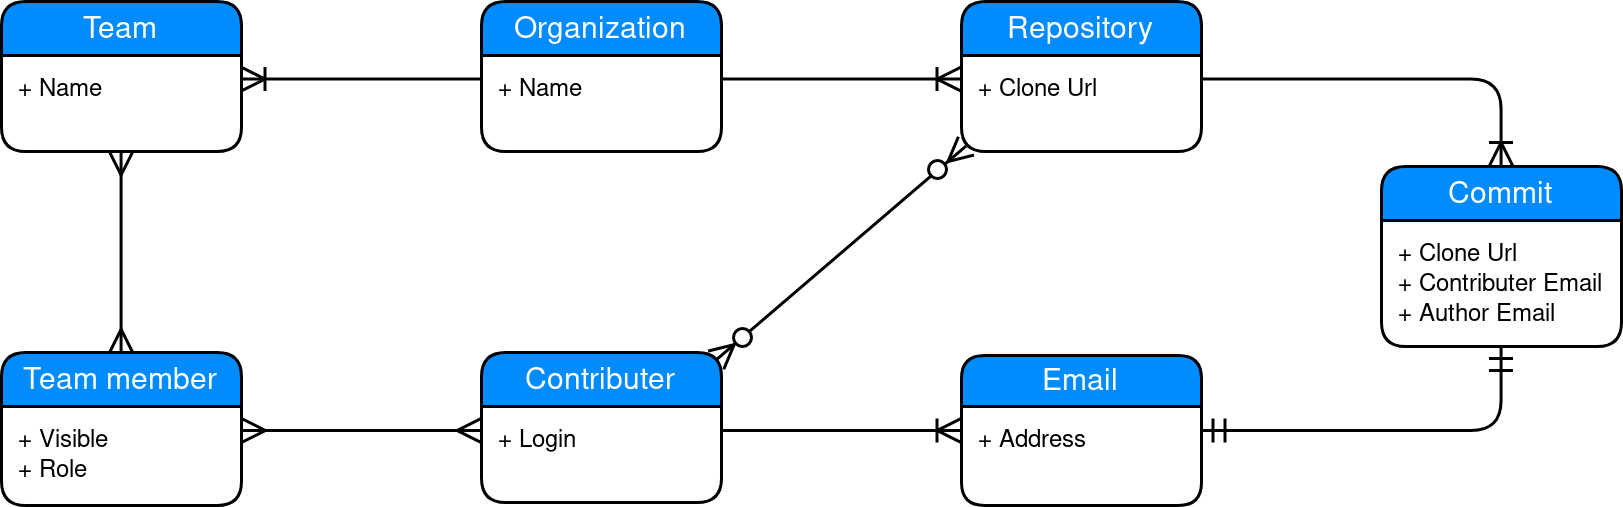
\includegraphics[scale=0.27]{./graphs/github-data-structure}
\centering
\caption{Simplified Github relationships.}\label{fig:github-relationship}
\end{figure}

\subsubsection{Github's features}
Github offers some features, which are convenient to for example find repositories a specific user contributed to or to find contributers which likely personally know each other.

\subsubsection{Stars}
The first feature is \emph{starring}. Every user can \emph{star} a repository to show that he likes a project.
The Github \ac{api} doesn't provide a method to get all repositories a user ever contributed to, it only allows to query the repositories actually owned or forked by a user, but it provides an endpoint to query all starred repositories of an user.
In case a user stars a repository he contributed to, whilst not owning it, it is possible to get this repository with this feature.
Of course it is still no reliable way to get all repositories a user contributed to, but it is a solution approach to get at least a few of them.

\subsection{Follower}
Another feature is \emph{following}. Every user can follow another user to get informed, if they do specific things like creating new repositories or starring repositories.
By getting the followers or following, one might catch some friends of the user.
It is also possible that a user follows the owner of a repository he contributed to.
By using this feature it is thereby possible to catch some additional contributed repositories as well some friends of the user.

\subsection{Organizations}\label{github-organization}
The third feature are \emph{organizations}.
An organization is used to host projects under an account which is not necessarily led by a single natural person, but rather supports roles with different permissions and team structures.

This feature provides us with some important ground truth, but sadly a lot of information is not visible, as users have to actively opt-in, if they want to be publicly displayed as a member of an organization.
Additionally team structures can only be examined, if one is a member of the organization.
Despite not knowing all members of an organization, we still get some useful information to estimate the tendency of precision of our knowledge extraction algorithms.
